\documentclass[9pt]{beamer}


\usepackage[english,russian]{babel}
\usepackage[utf8]{inputenc}
\usepackage{graphicx}
\usepackage{ragged2e}
\usepackage{textpos}
\usepackage{amsmath}
\usepackage{xcolor}
\usepackage[normalem]{ulem}
\usepackage{hhline}
\usepackage{colortbl}
\usepackage{array}
\graphicspath{{pictures/}}
\inputencoding{utf8}
\usepackage{geometry}
\parskip=0.1mm
\title{Шестая лаба на сто баллов.}
\author{ExcaliBBur\\ Павлов Александр}
\subtitle{Вариант №8}
\geometry{left=0mm,top=0mm,right=0.3mm}
\begin{document}
	\begin{frame}
		\titlepage
	\end{frame}
	\begin{frame}
	\begin{flushright}
	\vspace{1em}
		\large{\textcolor{blue}{П}рограммное обесп\textcolor{red}{$\acute{e}$}чение или обеспеч\textcolor{red}{$\acute{e}$}ние}
		\\ \rule{10cm}{0.4pt}
	\end{flushright}
	\begin{textblock*}{0mm}(0mm,-12mm)
		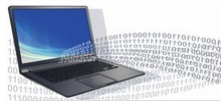
\includegraphics[scale=0.7]{balakshin.png}
	\end{textblock*}
\vspace{1.5em}
	$\left.
	\colorbox{gray!20}{
	\parbox{.8\linewidth}{
	\begin{enumerate}
		\scriptsize{\item Орфоэпический словарь (Аванесов, 1988): 
		обесп$\acute{e}$чение, ! не рек. обеспеч$\acute{e}$ние.
	\item Русское словесное ударение (Зарва, 2002): обесп$\acute{e}$чение [не обеспеч$\acute{e}$ние]
	\item Словарь трудностей произношения и ударения в современном русском языке (Горбачевич, 2002):обесп$\acute{e}$чение (не рекомендуется обеспеч$\acute{e}$ние)
	\item Учебный словарь трудностей произношения и ударения в современном русском языке (2004, Гостеева): Обесп$\acute{e}$чение. Не рек. обеспеч$\acute{e}$ние
	\item Современный толковый словарь русского языка (Ефремова, 2000): обесп$\acute{e}$чение; обеспеч$\acute{e}$ние разг.
	\item Давайте говорить правильно (Вербицкая, 2008): обесп$\acute{e}$чение, в проф. речи обеспеч$\acute{e}$ние}
	\end{enumerate}%
	}%
	}
	\right\} \small{\text{обесп$\acute{e}$чение}}$
	$\left.
	\colorbox{gray!20}{
	\parbox{.6\linewidth}{
	\begin{enumerate}
		\scriptsize{\item Большой толковый словарь (Кузнецов, 2009).
		\item Толковый словарь (Ожегов, 1992).
		\item Толковый словарь (Ушаков, 1940).
		\item Морфемно-орфографический словарь (Тихонов, 2002).
		\item Collins Russian Dictionary (2000).
		\item Онлайн-словарь \url{http://www.wiktionary.org}
		\item Онлайн-словарь \url{http://en.bab.la}
		\item Онлайн-словарь \url{http://ru.forvo.com}}
	\end{enumerate}%
	}%
	}
	\right\} \small{\text{обеспеч$\acute{e}$ние}}$
	$\left.
	\colorbox{gray!20}{
	\parbox{.6\linewidth}{
	\begin{enumerate}
		\scriptsize{\item Русский орфографический словарь (Лопатин, 2004).
\item Толковый словарь (Дмитриев, 2003).}
	\end{enumerate}%
	}%
	}
	\right\} \small{\text{обесп$\acute{e}$чение обеспеч$\acute{e}$ние}}$
	\end{frame}
	\begin{frame}
	\begin{flushright}
	\vspace{1em}
		\large{\textcolor{blue}{О}фисное программное обесп$\acute{e}$чение}
		\\ \rule{10cm}{0.4pt}
	\end{flushright}
	\begin{textblock*}{0mm}(0mm,-12mm)
		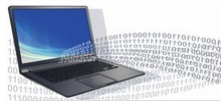
\includegraphics[scale=0.7]{balakshin.png}
	\end{textblock*}
\vspace{1.5em}
	К офисному программному обеспечению (ПО) относят наиболее часто
применяемые в офисной работе программы для редактирования электронных документов.
Существует более 30 серьёзных \textcolor{green} {офисных пакетов} разных производителей. Они различаются по
составу и функциональности, но почти во всех присутствуют следующие три обязательных
компонента:
	\begin{itemize}
		\item Текстовый процессор (текстовый редактор) – ТП.
		\item Электронная таблица (табличный процессор) – ЭТ.
		\item Программа подготовки презентаций – ПП.
	\end{itemize}
	\textcolor{green}{Форматы} файлов офисного ПО (наиболее популярные):
	\begin{itemize}
		\item ТП: doc, docx, odt
		\item ЭТ: xls, xlsx, ods
		\item ПП: ppt, pptx, odp
	\end{itemize}
	\textcolor{green}{Интересные факты}
	\begin{itemize}
		\item Форматы doc/xls/ppt до сих пор «закрыты» (по состоянию на 2017 год), хотя в разное время
компания Microsoft предоставляла временный и/или частичный доступ к ним.
		\item Форматы docx, odt, xlsx, ods, pptx, odp – это zip-архивы с xml- и медиафайлами.
		\item Криптографическая защита в doc, xls, ppt крайне слабая (даже для длинных паролей)
	\end{itemize}
	\end{frame}
	\begin{frame}
	\begin{flushright}
	\vspace{1em}
		\large{\textcolor{blue}{Н}аиболее популярные офисные пакеты}
		\\ \rule{10cm}{0.4pt}
	\end{flushright}
	\begin{textblock*}{0mm}(0mm,-12mm)
		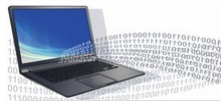
\includegraphics[scale=0.7]{balakshin.png}
	\end{textblock*}
	\begin{textblock*}{90mm}(41mm,-1mm)
	\scriptsize{Данные о популярности офисных пакетов получены с помощью анализа статистики,
собранной с помощью сайта trends.google.com. В таблице пакеты приведены по
убыванию популярности. Стоимость указана для desktop-версий.}
	\end{textblock*}
	\vspace{1em}
	\small{
	\begin{table}\centering
	\begin{tabular}{|>{\centering\arraybackslash}p{43mm}|>{\centering\arraybackslash}p{40mm}|>{\centering\arraybackslash}p{15mm}|>{\centering\arraybackslash}p{13mm}|}
	\hline
	 \rowcolor{black} 
	\textcolor{white}{\textbf{Название офисного пакета}} & \textcolor{white}					{\textbf{Особенности}} &\textcolor{white}{Примерная стоимость на 2020 год, руб.} & \textcolor{white}		{\textbf{Исходный код}} \\
	\hline
	\textcolor{green}{Google Docs,} Яндекс.Диск, Облако Mail.ru & Узкая ориентация на публичные облачные решения & бесплатно & закрытый \\ \hline
Microsoft Office (+ Office
365) &
Имеет \textcolor{green}{наиболее богатая функциональность,}
захватил > 90\% desktop-установок & 5000–17000& закрытый\\ \hline
\textcolor{green}{LibreOffice,} OpenOffice,
Calligra Suite &
Слабая поддержка одновременного
редактирования&
бесплатно &\textcolor{green}{открытый}\\ \hline
iWork& Узкая ориентация на технику
компании Apple& бесплатно &закрытый\\ \hline
WPS Office &Интерфейс идентичен Microsoft Office &3000-8000& закрытый\\ \hline
WordPerfect Office &Узкая ориентация на рынок персональных
компьютеров&
7000–28000 &закрытый\\ \hline
\textcolor{green}{OnlyOffice,} Feng Office &Приоритетная ориентация на частные и
публичные облачные решения& бесплатно*& \textcolor{green}{открытый}\\ \hline
	\end{tabular}
	\end{table}
	}
	\end{frame}
	\begin{frame}
	\begin{flushright}
	\vspace{1em}
		\large{\textcolor{blue}{Ф}ормат ODF и ГОСТ России}
		\\ \rule{10cm}{0.4pt}
	\end{flushright}
	\begin{textblock*}{0mm}(0mm,-12mm)
		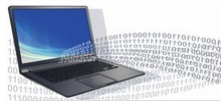
\includegraphics[scale=0.7]{balakshin.png}
	\end{textblock*}
	\vspace{2em}
	Открытый бесплатный формат \textcolor{green}{ODF} (Open Document Format) позволяет обеспечить возможность
долгосрочного хранения электронных документов без привязки к «капризам» конкретного
производителя офисного ПО. Стандарты ODF описывают 16 форматов файлов (документы,
картинки, таблицы, формулы, диаграммы), включая odt, ods, odp.\\
\textcolor{green}{Стандратизация ODF в России} (во многих других странах ситуация похожая)
	\begin{itemize}
	\item ODF 1.0 был описан и введён в действия по ГОСТ 26300-2010 (с 1 июня 2011 г.)
\item ГОСТ 26300-2010 должен использоваться для документооборота в госстр
\item Стандартизация ODF не означает навязывание LibreOffice/OpenOffice.
	\end{itemize}
\textcolor{green}{Проблемы ГОСТ 26300-2010}
	\begin{itemize}
	\item Текущая версия ODF уже 1.3 (в ней исправлены многие проблемы версии 1.0)
\item Не описаны спецификации скриптов и макросов.
\item Не описано применение цифровых подписей.
\item Не описан язык описания формул.
\item Не допускается использование таблиц в презентациях
	\end{itemize}
	\textcolor{green}{Спецификация ODF 1.3 (декабрь 2019), принят 21 января 2020: }
	\\
	\url{https://docs.oasis-open.org/office/OpenDocument/v1.3/cs01/}
	\end{frame}
	\begin{frame}
	\begin{flushright}
	\vspace{1em}
		\large{"\textcolor{blue}{П}родвинутые" функции текстовых процессоров и \\ электронных таблиц}
		\\ \rule{10cm}{0.4pt}
	\end{flushright}
	\begin{textblock*}{0mm}(0mm,-12mm)
		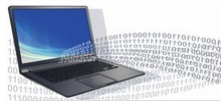
\includegraphics[scale=0.7]{balakshin.png}
	\end{textblock*}
	\vspace{2em}
	В школе офисные пакеты изучаются очень подробно. Однако есть ряд немаловажных
функций текстовых процессоров и электронных таблиц, о которых в школе почти не говорят.\\
	\textcolor{green}{Текстовый процессор}
	\begin{itemize}
	\item Концепция стилей для оформления текстового документа
\item Автонумерация рисунков, таблиц, формул
\item Макросы для автоматизации повторяющихся действий
\item Автозаполнение «мусорным» текстом
	\end{itemize}
	\textcolor{green}{Табличный процессор}
	\begin{itemize}
	\item Расчёт доверительного интервала
\item Фильтры содержимого таблиц
\item Запрет на ввод некорректных значений в ячейку.
\item Условное форматирование
\item Инструмент «Подбор параметра»
	\end{itemize}
	Рассматриваемые далее примеры выполнены в LibreOffice 5.1, однако в других офисных
пакетах есть аналогичные функции (даже их названия почти всегда дословно совпадают).
	\end{frame}
\end{document}